\documentclass[11pt]{article}

    \usepackage[breakable]{tcolorbox}
    \usepackage{parskip} % Stop auto-indenting (to mimic markdown behaviour)
    

    % Basic figure setup, for now with no caption control since it's done
    % automatically by Pandoc (which extracts ![](path) syntax from Markdown).
    \usepackage{graphicx}
    % Keep aspect ratio if custom image width or height is specified
    \setkeys{Gin}{keepaspectratio}
    % Maintain compatibility with old templates. Remove in nbconvert 6.0
    \let\Oldincludegraphics\includegraphics
    % Ensure that by default, figures have no caption (until we provide a
    % proper Figure object with a Caption API and a way to capture that
    % in the conversion process - todo).
    \usepackage{caption}
    \DeclareCaptionFormat{nocaption}{}
    \captionsetup{format=nocaption,aboveskip=0pt,belowskip=0pt}

    \usepackage{float}
    \floatplacement{figure}{H} % forces figures to be placed at the correct location
    \usepackage{xcolor} % Allow colors to be defined
    \usepackage{enumerate} % Needed for markdown enumerations to work
    \usepackage{geometry} % Used to adjust the document margins
    \usepackage{amsmath} % Equations
    \usepackage{amssymb} % Equations
    \usepackage{textcomp} % defines textquotesingle
    % Hack from http://tex.stackexchange.com/a/47451/13684:
    \AtBeginDocument{%
        \def\PYZsq{\textquotesingle}% Upright quotes in Pygmentized code
    }
    \usepackage{upquote} % Upright quotes for verbatim code
    \usepackage{eurosym} % defines \euro

    \usepackage{iftex}
    \ifPDFTeX
        \usepackage[T1]{fontenc}
        \IfFileExists{alphabeta.sty}{
              \usepackage{alphabeta}
          }{
              \usepackage[mathletters]{ucs}
              \usepackage[utf8x]{inputenc}
          }
    \else
        \usepackage{fontspec}
        \usepackage{unicode-math}
    \fi

    \usepackage{fancyvrb} % verbatim replacement that allows latex
    \usepackage{grffile} % extends the file name processing of package graphics
                         % to support a larger range
    \makeatletter % fix for old versions of grffile with XeLaTeX
    \@ifpackagelater{grffile}{2019/11/01}
    {
      % Do nothing on new versions
    }
    {
      \def\Gread@@xetex#1{%
        \IfFileExists{"\Gin@base".bb}%
        {\Gread@eps{\Gin@base.bb}}%
        {\Gread@@xetex@aux#1}%
      }
    }
    \makeatother
    \usepackage[Export]{adjustbox} % Used to constrain images to a maximum size
    \adjustboxset{max size={0.9\linewidth}{0.9\paperheight}}

    % The hyperref package gives us a pdf with properly built
    % internal navigation ('pdf bookmarks' for the table of contents,
    % internal cross-reference links, web links for URLs, etc.)
    \usepackage{hyperref}
    % The default LaTeX title has an obnoxious amount of whitespace. By default,
    % titling removes some of it. It also provides customization options.
    \usepackage{titling}
    \usepackage{longtable} % longtable support required by pandoc >1.10
    \usepackage{booktabs}  % table support for pandoc > 1.12.2
    \usepackage{array}     % table support for pandoc >= 2.11.3
    \usepackage{calc}      % table minipage width calculation for pandoc >= 2.11.1
    \usepackage[inline]{enumitem} % IRkernel/repr support (it uses the enumerate* environment)
    \usepackage[normalem]{ulem} % ulem is needed to support strikethroughs (\sout)
                                % normalem makes italics be italics, not underlines
    \usepackage{soul}      % strikethrough (\st) support for pandoc >= 3.0.0
    \usepackage{mathrsfs}
    

    
    % Colors for the hyperref package
    \definecolor{urlcolor}{rgb}{0,.145,.698}
    \definecolor{linkcolor}{rgb}{.71,0.21,0.01}
    \definecolor{citecolor}{rgb}{.12,.54,.11}

    % ANSI colors
    \definecolor{ansi-black}{HTML}{3E424D}
    \definecolor{ansi-black-intense}{HTML}{282C36}
    \definecolor{ansi-red}{HTML}{E75C58}
    \definecolor{ansi-red-intense}{HTML}{B22B31}
    \definecolor{ansi-green}{HTML}{00A250}
    \definecolor{ansi-green-intense}{HTML}{007427}
    \definecolor{ansi-yellow}{HTML}{DDB62B}
    \definecolor{ansi-yellow-intense}{HTML}{B27D12}
    \definecolor{ansi-blue}{HTML}{208FFB}
    \definecolor{ansi-blue-intense}{HTML}{0065CA}
    \definecolor{ansi-magenta}{HTML}{D160C4}
    \definecolor{ansi-magenta-intense}{HTML}{A03196}
    \definecolor{ansi-cyan}{HTML}{60C6C8}
    \definecolor{ansi-cyan-intense}{HTML}{258F8F}
    \definecolor{ansi-white}{HTML}{C5C1B4}
    \definecolor{ansi-white-intense}{HTML}{A1A6B2}
    \definecolor{ansi-default-inverse-fg}{HTML}{FFFFFF}
    \definecolor{ansi-default-inverse-bg}{HTML}{000000}

    % common color for the border for error outputs.
    \definecolor{outerrorbackground}{HTML}{FFDFDF}

    % commands and environments needed by pandoc snippets
    % extracted from the output of `pandoc -s`
    \providecommand{\tightlist}{%
      \setlength{\itemsep}{0pt}\setlength{\parskip}{0pt}}
    \DefineVerbatimEnvironment{Highlighting}{Verbatim}{commandchars=\\\{\}}
    % Add ',fontsize=\small' for more characters per line
    \newenvironment{Shaded}{}{}
    \newcommand{\KeywordTok}[1]{\textcolor[rgb]{0.00,0.44,0.13}{\textbf{{#1}}}}
    \newcommand{\DataTypeTok}[1]{\textcolor[rgb]{0.56,0.13,0.00}{{#1}}}
    \newcommand{\DecValTok}[1]{\textcolor[rgb]{0.25,0.63,0.44}{{#1}}}
    \newcommand{\BaseNTok}[1]{\textcolor[rgb]{0.25,0.63,0.44}{{#1}}}
    \newcommand{\FloatTok}[1]{\textcolor[rgb]{0.25,0.63,0.44}{{#1}}}
    \newcommand{\CharTok}[1]{\textcolor[rgb]{0.25,0.44,0.63}{{#1}}}
    \newcommand{\StringTok}[1]{\textcolor[rgb]{0.25,0.44,0.63}{{#1}}}
    \newcommand{\CommentTok}[1]{\textcolor[rgb]{0.38,0.63,0.69}{\textit{{#1}}}}
    \newcommand{\OtherTok}[1]{\textcolor[rgb]{0.00,0.44,0.13}{{#1}}}
    \newcommand{\AlertTok}[1]{\textcolor[rgb]{1.00,0.00,0.00}{\textbf{{#1}}}}
    \newcommand{\FunctionTok}[1]{\textcolor[rgb]{0.02,0.16,0.49}{{#1}}}
    \newcommand{\RegionMarkerTok}[1]{{#1}}
    \newcommand{\ErrorTok}[1]{\textcolor[rgb]{1.00,0.00,0.00}{\textbf{{#1}}}}
    \newcommand{\NormalTok}[1]{{#1}}

    % Additional commands for more recent versions of Pandoc
    \newcommand{\ConstantTok}[1]{\textcolor[rgb]{0.53,0.00,0.00}{{#1}}}
    \newcommand{\SpecialCharTok}[1]{\textcolor[rgb]{0.25,0.44,0.63}{{#1}}}
    \newcommand{\VerbatimStringTok}[1]{\textcolor[rgb]{0.25,0.44,0.63}{{#1}}}
    \newcommand{\SpecialStringTok}[1]{\textcolor[rgb]{0.73,0.40,0.53}{{#1}}}
    \newcommand{\ImportTok}[1]{{#1}}
    \newcommand{\DocumentationTok}[1]{\textcolor[rgb]{0.73,0.13,0.13}{\textit{{#1}}}}
    \newcommand{\AnnotationTok}[1]{\textcolor[rgb]{0.38,0.63,0.69}{\textbf{\textit{{#1}}}}}
    \newcommand{\CommentVarTok}[1]{\textcolor[rgb]{0.38,0.63,0.69}{\textbf{\textit{{#1}}}}}
    \newcommand{\VariableTok}[1]{\textcolor[rgb]{0.10,0.09,0.49}{{#1}}}
    \newcommand{\ControlFlowTok}[1]{\textcolor[rgb]{0.00,0.44,0.13}{\textbf{{#1}}}}
    \newcommand{\OperatorTok}[1]{\textcolor[rgb]{0.40,0.40,0.40}{{#1}}}
    \newcommand{\BuiltInTok}[1]{{#1}}
    \newcommand{\ExtensionTok}[1]{{#1}}
    \newcommand{\PreprocessorTok}[1]{\textcolor[rgb]{0.74,0.48,0.00}{{#1}}}
    \newcommand{\AttributeTok}[1]{\textcolor[rgb]{0.49,0.56,0.16}{{#1}}}
    \newcommand{\InformationTok}[1]{\textcolor[rgb]{0.38,0.63,0.69}{\textbf{\textit{{#1}}}}}
    \newcommand{\WarningTok}[1]{\textcolor[rgb]{0.38,0.63,0.69}{\textbf{\textit{{#1}}}}}
    \makeatletter
    \newsavebox\pandoc@box
    \newcommand*\pandocbounded[1]{%
      \sbox\pandoc@box{#1}%
      % scaling factors for width and height
      \Gscale@div\@tempa\textheight{\dimexpr\ht\pandoc@box+\dp\pandoc@box\relax}%
      \Gscale@div\@tempb\linewidth{\wd\pandoc@box}%
      % select the smaller of both
      \ifdim\@tempb\p@<\@tempa\p@
        \let\@tempa\@tempb
      \fi
      % scaling accordingly (\@tempa < 1)
      \ifdim\@tempa\p@<\p@
        \scalebox{\@tempa}{\usebox\pandoc@box}%
      % scaling not needed, use as it is
      \else
        \usebox{\pandoc@box}%
      \fi
    }
    \makeatother

    % Define a nice break command that doesn't care if a line doesn't already
    % exist.
    \def\br{\hspace*{\fill} \\* }
    % Math Jax compatibility definitions
    \def\gt{>}
    \def\lt{<}
    \let\Oldtex\TeX
    \let\Oldlatex\LaTeX
    \renewcommand{\TeX}{\textrm{\Oldtex}}
    \renewcommand{\LaTeX}{\textrm{\Oldlatex}}
    % Document parameters
    % Document title
    \title{hw5}
    
    
    
    
    
    
    
% Pygments definitions
\makeatletter
\def\PY@reset{\let\PY@it=\relax \let\PY@bf=\relax%
    \let\PY@ul=\relax \let\PY@tc=\relax%
    \let\PY@bc=\relax \let\PY@ff=\relax}
\def\PY@tok#1{\csname PY@tok@#1\endcsname}
\def\PY@toks#1+{\ifx\relax#1\empty\else%
    \PY@tok{#1}\expandafter\PY@toks\fi}
\def\PY@do#1{\PY@bc{\PY@tc{\PY@ul{%
    \PY@it{\PY@bf{\PY@ff{#1}}}}}}}
\def\PY#1#2{\PY@reset\PY@toks#1+\relax+\PY@do{#2}}

\@namedef{PY@tok@w}{\def\PY@tc##1{\textcolor[rgb]{0.73,0.73,0.73}{##1}}}
\@namedef{PY@tok@c}{\let\PY@it=\textit\def\PY@tc##1{\textcolor[rgb]{0.24,0.48,0.48}{##1}}}
\@namedef{PY@tok@cp}{\def\PY@tc##1{\textcolor[rgb]{0.61,0.40,0.00}{##1}}}
\@namedef{PY@tok@k}{\let\PY@bf=\textbf\def\PY@tc##1{\textcolor[rgb]{0.00,0.50,0.00}{##1}}}
\@namedef{PY@tok@kp}{\def\PY@tc##1{\textcolor[rgb]{0.00,0.50,0.00}{##1}}}
\@namedef{PY@tok@kt}{\def\PY@tc##1{\textcolor[rgb]{0.69,0.00,0.25}{##1}}}
\@namedef{PY@tok@o}{\def\PY@tc##1{\textcolor[rgb]{0.40,0.40,0.40}{##1}}}
\@namedef{PY@tok@ow}{\let\PY@bf=\textbf\def\PY@tc##1{\textcolor[rgb]{0.67,0.13,1.00}{##1}}}
\@namedef{PY@tok@nb}{\def\PY@tc##1{\textcolor[rgb]{0.00,0.50,0.00}{##1}}}
\@namedef{PY@tok@nf}{\def\PY@tc##1{\textcolor[rgb]{0.00,0.00,1.00}{##1}}}
\@namedef{PY@tok@nc}{\let\PY@bf=\textbf\def\PY@tc##1{\textcolor[rgb]{0.00,0.00,1.00}{##1}}}
\@namedef{PY@tok@nn}{\let\PY@bf=\textbf\def\PY@tc##1{\textcolor[rgb]{0.00,0.00,1.00}{##1}}}
\@namedef{PY@tok@ne}{\let\PY@bf=\textbf\def\PY@tc##1{\textcolor[rgb]{0.80,0.25,0.22}{##1}}}
\@namedef{PY@tok@nv}{\def\PY@tc##1{\textcolor[rgb]{0.10,0.09,0.49}{##1}}}
\@namedef{PY@tok@no}{\def\PY@tc##1{\textcolor[rgb]{0.53,0.00,0.00}{##1}}}
\@namedef{PY@tok@nl}{\def\PY@tc##1{\textcolor[rgb]{0.46,0.46,0.00}{##1}}}
\@namedef{PY@tok@ni}{\let\PY@bf=\textbf\def\PY@tc##1{\textcolor[rgb]{0.44,0.44,0.44}{##1}}}
\@namedef{PY@tok@na}{\def\PY@tc##1{\textcolor[rgb]{0.41,0.47,0.13}{##1}}}
\@namedef{PY@tok@nt}{\let\PY@bf=\textbf\def\PY@tc##1{\textcolor[rgb]{0.00,0.50,0.00}{##1}}}
\@namedef{PY@tok@nd}{\def\PY@tc##1{\textcolor[rgb]{0.67,0.13,1.00}{##1}}}
\@namedef{PY@tok@s}{\def\PY@tc##1{\textcolor[rgb]{0.73,0.13,0.13}{##1}}}
\@namedef{PY@tok@sd}{\let\PY@it=\textit\def\PY@tc##1{\textcolor[rgb]{0.73,0.13,0.13}{##1}}}
\@namedef{PY@tok@si}{\let\PY@bf=\textbf\def\PY@tc##1{\textcolor[rgb]{0.64,0.35,0.47}{##1}}}
\@namedef{PY@tok@se}{\let\PY@bf=\textbf\def\PY@tc##1{\textcolor[rgb]{0.67,0.36,0.12}{##1}}}
\@namedef{PY@tok@sr}{\def\PY@tc##1{\textcolor[rgb]{0.64,0.35,0.47}{##1}}}
\@namedef{PY@tok@ss}{\def\PY@tc##1{\textcolor[rgb]{0.10,0.09,0.49}{##1}}}
\@namedef{PY@tok@sx}{\def\PY@tc##1{\textcolor[rgb]{0.00,0.50,0.00}{##1}}}
\@namedef{PY@tok@m}{\def\PY@tc##1{\textcolor[rgb]{0.40,0.40,0.40}{##1}}}
\@namedef{PY@tok@gh}{\let\PY@bf=\textbf\def\PY@tc##1{\textcolor[rgb]{0.00,0.00,0.50}{##1}}}
\@namedef{PY@tok@gu}{\let\PY@bf=\textbf\def\PY@tc##1{\textcolor[rgb]{0.50,0.00,0.50}{##1}}}
\@namedef{PY@tok@gd}{\def\PY@tc##1{\textcolor[rgb]{0.63,0.00,0.00}{##1}}}
\@namedef{PY@tok@gi}{\def\PY@tc##1{\textcolor[rgb]{0.00,0.52,0.00}{##1}}}
\@namedef{PY@tok@gr}{\def\PY@tc##1{\textcolor[rgb]{0.89,0.00,0.00}{##1}}}
\@namedef{PY@tok@ge}{\let\PY@it=\textit}
\@namedef{PY@tok@gs}{\let\PY@bf=\textbf}
\@namedef{PY@tok@ges}{\let\PY@bf=\textbf\let\PY@it=\textit}
\@namedef{PY@tok@gp}{\let\PY@bf=\textbf\def\PY@tc##1{\textcolor[rgb]{0.00,0.00,0.50}{##1}}}
\@namedef{PY@tok@go}{\def\PY@tc##1{\textcolor[rgb]{0.44,0.44,0.44}{##1}}}
\@namedef{PY@tok@gt}{\def\PY@tc##1{\textcolor[rgb]{0.00,0.27,0.87}{##1}}}
\@namedef{PY@tok@err}{\def\PY@bc##1{{\setlength{\fboxsep}{\string -\fboxrule}\fcolorbox[rgb]{1.00,0.00,0.00}{1,1,1}{\strut ##1}}}}
\@namedef{PY@tok@kc}{\let\PY@bf=\textbf\def\PY@tc##1{\textcolor[rgb]{0.00,0.50,0.00}{##1}}}
\@namedef{PY@tok@kd}{\let\PY@bf=\textbf\def\PY@tc##1{\textcolor[rgb]{0.00,0.50,0.00}{##1}}}
\@namedef{PY@tok@kn}{\let\PY@bf=\textbf\def\PY@tc##1{\textcolor[rgb]{0.00,0.50,0.00}{##1}}}
\@namedef{PY@tok@kr}{\let\PY@bf=\textbf\def\PY@tc##1{\textcolor[rgb]{0.00,0.50,0.00}{##1}}}
\@namedef{PY@tok@bp}{\def\PY@tc##1{\textcolor[rgb]{0.00,0.50,0.00}{##1}}}
\@namedef{PY@tok@fm}{\def\PY@tc##1{\textcolor[rgb]{0.00,0.00,1.00}{##1}}}
\@namedef{PY@tok@vc}{\def\PY@tc##1{\textcolor[rgb]{0.10,0.09,0.49}{##1}}}
\@namedef{PY@tok@vg}{\def\PY@tc##1{\textcolor[rgb]{0.10,0.09,0.49}{##1}}}
\@namedef{PY@tok@vi}{\def\PY@tc##1{\textcolor[rgb]{0.10,0.09,0.49}{##1}}}
\@namedef{PY@tok@vm}{\def\PY@tc##1{\textcolor[rgb]{0.10,0.09,0.49}{##1}}}
\@namedef{PY@tok@sa}{\def\PY@tc##1{\textcolor[rgb]{0.73,0.13,0.13}{##1}}}
\@namedef{PY@tok@sb}{\def\PY@tc##1{\textcolor[rgb]{0.73,0.13,0.13}{##1}}}
\@namedef{PY@tok@sc}{\def\PY@tc##1{\textcolor[rgb]{0.73,0.13,0.13}{##1}}}
\@namedef{PY@tok@dl}{\def\PY@tc##1{\textcolor[rgb]{0.73,0.13,0.13}{##1}}}
\@namedef{PY@tok@s2}{\def\PY@tc##1{\textcolor[rgb]{0.73,0.13,0.13}{##1}}}
\@namedef{PY@tok@sh}{\def\PY@tc##1{\textcolor[rgb]{0.73,0.13,0.13}{##1}}}
\@namedef{PY@tok@s1}{\def\PY@tc##1{\textcolor[rgb]{0.73,0.13,0.13}{##1}}}
\@namedef{PY@tok@mb}{\def\PY@tc##1{\textcolor[rgb]{0.40,0.40,0.40}{##1}}}
\@namedef{PY@tok@mf}{\def\PY@tc##1{\textcolor[rgb]{0.40,0.40,0.40}{##1}}}
\@namedef{PY@tok@mh}{\def\PY@tc##1{\textcolor[rgb]{0.40,0.40,0.40}{##1}}}
\@namedef{PY@tok@mi}{\def\PY@tc##1{\textcolor[rgb]{0.40,0.40,0.40}{##1}}}
\@namedef{PY@tok@il}{\def\PY@tc##1{\textcolor[rgb]{0.40,0.40,0.40}{##1}}}
\@namedef{PY@tok@mo}{\def\PY@tc##1{\textcolor[rgb]{0.40,0.40,0.40}{##1}}}
\@namedef{PY@tok@ch}{\let\PY@it=\textit\def\PY@tc##1{\textcolor[rgb]{0.24,0.48,0.48}{##1}}}
\@namedef{PY@tok@cm}{\let\PY@it=\textit\def\PY@tc##1{\textcolor[rgb]{0.24,0.48,0.48}{##1}}}
\@namedef{PY@tok@cpf}{\let\PY@it=\textit\def\PY@tc##1{\textcolor[rgb]{0.24,0.48,0.48}{##1}}}
\@namedef{PY@tok@c1}{\let\PY@it=\textit\def\PY@tc##1{\textcolor[rgb]{0.24,0.48,0.48}{##1}}}
\@namedef{PY@tok@cs}{\let\PY@it=\textit\def\PY@tc##1{\textcolor[rgb]{0.24,0.48,0.48}{##1}}}

\def\PYZbs{\char`\\}
\def\PYZus{\char`\_}
\def\PYZob{\char`\{}
\def\PYZcb{\char`\}}
\def\PYZca{\char`\^}
\def\PYZam{\char`\&}
\def\PYZlt{\char`\<}
\def\PYZgt{\char`\>}
\def\PYZsh{\char`\#}
\def\PYZpc{\char`\%}
\def\PYZdl{\char`\$}
\def\PYZhy{\char`\-}
\def\PYZsq{\char`\'}
\def\PYZdq{\char`\"}
\def\PYZti{\char`\~}
% for compatibility with earlier versions
\def\PYZat{@}
\def\PYZlb{[}
\def\PYZrb{]}
\makeatother


    % For linebreaks inside Verbatim environment from package fancyvrb.
    \makeatletter
        \newbox\Wrappedcontinuationbox
        \newbox\Wrappedvisiblespacebox
        \newcommand*\Wrappedvisiblespace {\textcolor{red}{\textvisiblespace}}
        \newcommand*\Wrappedcontinuationsymbol {\textcolor{red}{\llap{\tiny$\m@th\hookrightarrow$}}}
        \newcommand*\Wrappedcontinuationindent {3ex }
        \newcommand*\Wrappedafterbreak {\kern\Wrappedcontinuationindent\copy\Wrappedcontinuationbox}
        % Take advantage of the already applied Pygments mark-up to insert
        % potential linebreaks for TeX processing.
        %        {, <, #, %, $, ' and ": go to next line.
        %        _, }, ^, &, >, - and ~: stay at end of broken line.
        % Use of \textquotesingle for straight quote.
        \newcommand*\Wrappedbreaksatspecials {%
            \def\PYGZus{\discretionary{\char`\_}{\Wrappedafterbreak}{\char`\_}}%
            \def\PYGZob{\discretionary{}{\Wrappedafterbreak\char`\{}{\char`\{}}%
            \def\PYGZcb{\discretionary{\char`\}}{\Wrappedafterbreak}{\char`\}}}%
            \def\PYGZca{\discretionary{\char`\^}{\Wrappedafterbreak}{\char`\^}}%
            \def\PYGZam{\discretionary{\char`\&}{\Wrappedafterbreak}{\char`\&}}%
            \def\PYGZlt{\discretionary{}{\Wrappedafterbreak\char`\<}{\char`\<}}%
            \def\PYGZgt{\discretionary{\char`\>}{\Wrappedafterbreak}{\char`\>}}%
            \def\PYGZsh{\discretionary{}{\Wrappedafterbreak\char`\#}{\char`\#}}%
            \def\PYGZpc{\discretionary{}{\Wrappedafterbreak\char`\%}{\char`\%}}%
            \def\PYGZdl{\discretionary{}{\Wrappedafterbreak\char`\$}{\char`\$}}%
            \def\PYGZhy{\discretionary{\char`\-}{\Wrappedafterbreak}{\char`\-}}%
            \def\PYGZsq{\discretionary{}{\Wrappedafterbreak\textquotesingle}{\textquotesingle}}%
            \def\PYGZdq{\discretionary{}{\Wrappedafterbreak\char`\"}{\char`\"}}%
            \def\PYGZti{\discretionary{\char`\~}{\Wrappedafterbreak}{\char`\~}}%
        }
        % Some characters . , ; ? ! / are not pygmentized.
        % This macro makes them "active" and they will insert potential linebreaks
        \newcommand*\Wrappedbreaksatpunct {%
            \lccode`\~`\.\lowercase{\def~}{\discretionary{\hbox{\char`\.}}{\Wrappedafterbreak}{\hbox{\char`\.}}}%
            \lccode`\~`\,\lowercase{\def~}{\discretionary{\hbox{\char`\,}}{\Wrappedafterbreak}{\hbox{\char`\,}}}%
            \lccode`\~`\;\lowercase{\def~}{\discretionary{\hbox{\char`\;}}{\Wrappedafterbreak}{\hbox{\char`\;}}}%
            \lccode`\~`\:\lowercase{\def~}{\discretionary{\hbox{\char`\:}}{\Wrappedafterbreak}{\hbox{\char`\:}}}%
            \lccode`\~`\?\lowercase{\def~}{\discretionary{\hbox{\char`\?}}{\Wrappedafterbreak}{\hbox{\char`\?}}}%
            \lccode`\~`\!\lowercase{\def~}{\discretionary{\hbox{\char`\!}}{\Wrappedafterbreak}{\hbox{\char`\!}}}%
            \lccode`\~`\/\lowercase{\def~}{\discretionary{\hbox{\char`\/}}{\Wrappedafterbreak}{\hbox{\char`\/}}}%
            \catcode`\.\active
            \catcode`\,\active
            \catcode`\;\active
            \catcode`\:\active
            \catcode`\?\active
            \catcode`\!\active
            \catcode`\/\active
            \lccode`\~`\~
        }
    \makeatother

    \let\OriginalVerbatim=\Verbatim
    \makeatletter
    \renewcommand{\Verbatim}[1][1]{%
        %\parskip\z@skip
        \sbox\Wrappedcontinuationbox {\Wrappedcontinuationsymbol}%
        \sbox\Wrappedvisiblespacebox {\FV@SetupFont\Wrappedvisiblespace}%
        \def\FancyVerbFormatLine ##1{\hsize\linewidth
            \vtop{\raggedright\hyphenpenalty\z@\exhyphenpenalty\z@
                \doublehyphendemerits\z@\finalhyphendemerits\z@
                \strut ##1\strut}%
        }%
        % If the linebreak is at a space, the latter will be displayed as visible
        % space at end of first line, and a continuation symbol starts next line.
        % Stretch/shrink are however usually zero for typewriter font.
        \def\FV@Space {%
            \nobreak\hskip\z@ plus\fontdimen3\font minus\fontdimen4\font
            \discretionary{\copy\Wrappedvisiblespacebox}{\Wrappedafterbreak}
            {\kern\fontdimen2\font}%
        }%

        % Allow breaks at special characters using \PYG... macros.
        \Wrappedbreaksatspecials
        % Breaks at punctuation characters . , ; ? ! and / need catcode=\active
        \OriginalVerbatim[#1,codes*=\Wrappedbreaksatpunct]%
    }
    \makeatother

    % Exact colors from NB
    \definecolor{incolor}{HTML}{303F9F}
    \definecolor{outcolor}{HTML}{D84315}
    \definecolor{cellborder}{HTML}{CFCFCF}
    \definecolor{cellbackground}{HTML}{F7F7F7}

    % prompt
    \makeatletter
    \newcommand{\boxspacing}{\kern\kvtcb@left@rule\kern\kvtcb@boxsep}
    \makeatother
    \newcommand{\prompt}[4]{
        {\ttfamily\llap{{\color{#2}[#3]:\hspace{3pt}#4}}\vspace{-\baselineskip}}
    }
    

    
    % Prevent overflowing lines due to hard-to-break entities
    \sloppy
    % Setup hyperref package
    \hypersetup{
      breaklinks=true,  % so long urls are correctly broken across lines
      colorlinks=true,
      urlcolor=urlcolor,
      linkcolor=linkcolor,
      citecolor=citecolor,
      }
    % Slightly bigger margins than the latex defaults
    
    \geometry{verbose,tmargin=1in,bmargin=1in,lmargin=1in,rmargin=1in}
    
    

\begin{document}
    
    \maketitle
    
    

    
    

    \section{Homework 5 (Due 14 Mar)}\label{homework-5-due-14-mar}

\textbf{Due 14 Mar (midnight)}

Total points: 100

    \begin{tcolorbox}[breakable, size=fbox, boxrule=1pt, pad at break*=1mm,colback=cellbackground, colframe=cellborder]
\prompt{In}{incolor}{ }{\boxspacing}
\begin{Verbatim}[commandchars=\\\{\}]
\PY{k+kn}{import}\PY{+w}{ }\PY{n+nn}{numpy}\PY{+w}{ }\PY{k}{as}\PY{+w}{ }\PY{n+nn}{np}
\PY{k+kn}{from}\PY{+w}{ }\PY{n+nn}{math}\PY{+w}{ }\PY{k+kn}{import} \PY{o}{*}
\PY{k+kn}{import}\PY{+w}{ }\PY{n+nn}{matplotlib}\PY{n+nn}{.}\PY{n+nn}{pyplot}\PY{+w}{ }\PY{k}{as}\PY{+w}{ }\PY{n+nn}{plt}
\PY{k+kn}{import}\PY{+w}{ }\PY{n+nn}{pandas}\PY{+w}{ }\PY{k}{as}\PY{+w}{ }\PY{n+nn}{pd}
\PY{o}{\PYZpc{}}\PY{k}{matplotlib} inline
\PY{n}{plt}\PY{o}{.}\PY{n}{style}\PY{o}{.}\PY{n}{use}\PY{p}{(}\PY{l+s+s1}{\PYZsq{}}\PY{l+s+s1}{seaborn\PYZhy{}v0\PYZus{}8\PYZhy{}colorblind}\PY{l+s+s1}{\PYZsq{}}\PY{p}{)}
\end{Verbatim}
\end{tcolorbox}

    \subsubsection{Exercise 1 (10 pt), SHO and Conservation of
Energy}\label{exercise-1-10-pt-sho-and-conservation-of-energy}

Consider the standard harmonic oscillator with a mass \(m\) attached to
a horizontal spring with spring constant \(k\). It is constrained to
move in the \(x\) direction only and there is no friction present. With
the equilibrium position as \(x=0\), then the potential energy is
\(U(x)=\frac{1}{2}kx^2\).

We give the oscillator a little kick at \(t=0\) and let it go. It
reaches a maximum distance of \(A\) from the equilibrium position.

\begin{itemize}
\tightlist
\item
  1a (2pt) Write down the conservation of energy equation and find the
  velocity as a function of position (i.e., find \(\dot{x}(x)\)).
\end{itemize}

    \begin{itemize}
\tightlist
\item
  1b (4pt) Construct the integral for the time it takes for the
  oscillator from \(x=0\) to any position \(x\).
\end{itemize}

    \begin{itemize}
\tightlist
\item
  1c (4pt) Use the integral to find \(x(t)\) and show that the period of
  the oscillator is \(T=2\pi\sqrt{m/k}\).
\end{itemize}

    \subsubsection{Exercise 2 (10pt), Kid's toy and stable
equilibrium}\label{exercise-2-10pt-kids-toy-and-stable-equilibrium}

A toy is made from a cylinder mounted on a hemisphere as shown in the
figure below. The hemisphere has a radius of \(R\) and the center of
mass of the whole toy is \(h\) above the ground.

\begin{figure}
\centering
\pandocbounded{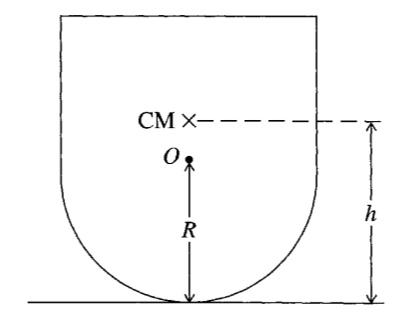
\includegraphics[keepaspectratio,alt={toy}]{/Users/caballero/repos/teaching/modern-classical-mechanics/content/images/activities/5.2-kid_toy.png}}
\caption{toy}
\end{figure}

\begin{itemize}
\tightlist
\item
  2a (2pt) Find the height of the center of mass of the toy as a
  function of the angle \(\theta\), measured from the vertical.
\end{itemize}

    \begin{itemize}
\tightlist
\item
  2b (3pt) Use this to find the gravitational potential energy
  \(U(\theta)\). Show in a figure how the potential energy varies with
  \(\theta\). Note that \(h/R\) becomes an important parameter. For
  different choices of \(h/R\) do the equilibrium points change? How?
\end{itemize}

    \begin{itemize}
\tightlist
\item
  2c (5pt) For which values of \(R\) and \(h\) is the toy in stable
  equilibrium so that it does not fall over? Does it fit with your
  graphical analysis? Why does this make sense to you? Or how would you
  explain it to a friend?
\end{itemize}

    \subsubsection{Exercise 3 (15pt), ``Generic'' 1D
motion}\label{exercise-3-15pt-generic-1d-motion}

We will eventually learn how to solve for equations of motion for
generalized coordinates. That work requires us to think about the forces
and constraints on a system. Here we will consider a particle moving
along a curved path to begin to think about how to describe the motion
of a particle in a more general way.

\begin{figure}
\centering
\pandocbounded{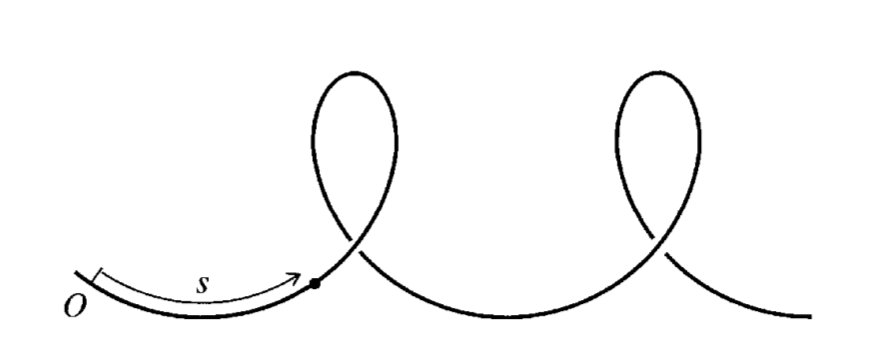
\includegraphics[keepaspectratio,alt={curved-path}]{/Users/caballero/repos/teaching/modern-classical-mechanics/content/images/activities/5.3-curved_path.png}}
\caption{curved-path}
\end{figure}

A bead follows the curved path above, you can imagine it is a wire or a
track, and the bead is constrained to move along the path. The bead's
position is described by its distance along the path, \(s\) as measured
from the origin \(O\). The \(\hat{s}\) direction is always along the
path - that is, it's always tangent to the wire.

\begin{itemize}
\item
  3a (3pt) Let's start by writing the velocity \(\mathbf{v}\) in terms
  of its Cartesian components (e.g., \(dx/dt\)) and find it's magnitude
  (\(v\)). How does this approach seem given the shape of the wire? Do
  you think we have chosen a good set of coordinates?
\item
  3b (4pt) Instead, consider the coordinate system
  \(\langle \hat{s}, \hat{s}_{\perp}\rangle\). That is the the direction
  along the path and the direction perpendicular to it (assume we are
  solving this in a plane for the moment). Use this coordinate system to
  show that bead's speed is given by \(v=\dot{s}\), that is there is no
  dependence of the speed on the \(\hat{s}_{\perp}\) component of
  \(\vec{v}\). How might this be a better choice?
\end{itemize}

    \begin{itemize}
\tightlist
\item
  3c (4pt) Still using this coordinate system, prove that the tangential
  component of the net force (\(F_{||}\), ``parallel'' to the motion) on
  the bead is \(m\ddot{s}\).
\end{itemize}

    There is a force due to the wire (\(\mathbf{F}_w\)) that ensures the
bead stays on the path. It is not in the direction of the path (i.e.,
friction), only perpendicular to the wire. Assume all other forces are
conservative (i.e., can be derived from a generic potential
\(-\nabla U\)).

\begin{itemize}
\tightlist
\item
  3d (4pt) Show that the tangential component of the net force due to
  the wire is \(-\frac{dU}{ds}\).
\end{itemize}

This 1D concept extends to multiple dimensions and can help us
understand the Lagrangian method of solving for the equations of motion.

```\{admonition\} Projection of a gradient :class: info

We can calculate the projection for a generic potential in a particular
Cartesian direction.

\[\nabla U(\vec{r}) \cdot \hat{x} = \langle \dfrac{dU(\vec{r})}{dx}, \dfrac{dU(\vec{r})}{dy}, \dfrac{dU(\vec{r})}{dz} \rangle \cdot \langle 1,0,0 \rangle = \dfrac{dU(\vec{r})}{dx}\]

Ultimately, the projection is the what the potential changes with
respect to the projection direction. ```

    \subsubsection{Exercise 4 (15pt), Another 1-D conservative system; baby
bifurcations}\label{exercise-4-15pt-another-1-d-conservative-system-baby-bifurcations}

The apparatus below is a massless wheel of radius \(R\) that is mounted
to a frictionless axle. A small, dense piece of clay with mass \(M\) is
glued to edge of the wheel as shown. Another mass \(m\) hangs from a
massless string that is wrapped around the wheel. We can assume the
string is inextensible and does not slip, and the system is in a uniform
gravitational field.

\begin{figure}
\centering
\pandocbounded{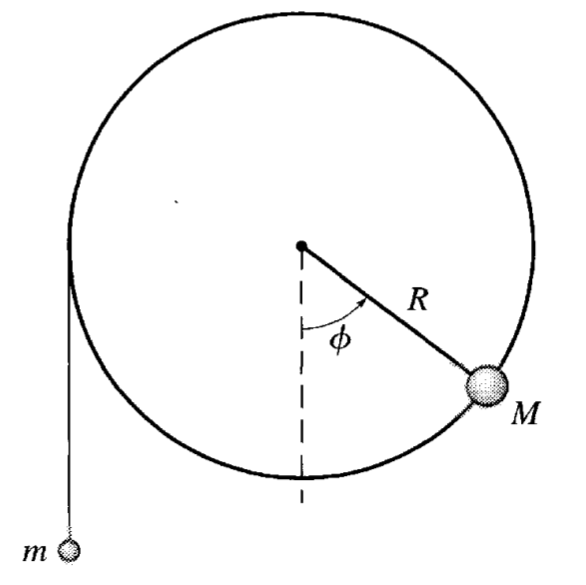
\includegraphics[keepaspectratio,alt={apparatus}]{/Users/caballero/repos/teaching/modern-classical-mechanics/content/images/activities/5.4-apparatus.png}}
\caption{apparatus}
\end{figure}

We can show that this complicated system is still one-dimensional (at
least in space) and then we can see the effects of parameters like
\(m/M\).

\begin{itemize}
\tightlist
\item
  4a (3pt) In terms of the rotation angle \(\phi\) of the wheel, write
  down the total potential energy \(U(\phi)\) of the system of both
  masses. Take note of any constraints that you use to write this as a
  1D problem. When working this kind of problem, every object-Earth pair
  has gravitational potential energy and we must have the same zero of
  potential energy for every pair.
\end{itemize}

    \begin{itemize}
\tightlist
\item
  4b (2pt) Use this potential energy to find values of \(m\) and \(M\)
  for which there are ``fixed points'', ``critical points'', or what we
  sometimes call ``equilibrium points''. The language we use comes from
  different fields, but the concept is the same. What is the condition
  for the existence of any critical points?
\end{itemize}

    \begin{itemize}
\tightlist
\item
  4c (3pt) Describe the fixed points, determine their stability, and
  explain why they make sense in terms of the expected motion.
\end{itemize}

    \begin{itemize}
\tightlist
\item
  4d (5pt) Plot the potential energy for two different values of \(m/M\)
  and explain the differences in the potential energy graphs. Consider
  cases when you observe very different motion. Think about an initial
  condition where the mass \(m\) is at rest and the wheel is at rest.
  What happens when you release the mass \(m\) for your two cases?
\end{itemize}

    \begin{itemize}
\tightlist
\item
  4e (2pt) Determine the value of \(m/M\) for which the system begins to
  exhibit oscillations (if released from \(\phi=0\)).
\end{itemize}

The value of \(m/M\) is a dimensionless quantity that characterizes the
system. In a dynamical system, we think of it as a parameter that can
change the qualitative behavior of the system. Such parameters can lead
us to
\href{https://en.wikipedia.org/wiki/Bifurcation_theory}{bifurcations},
\href{https://en.wikipedia.org/wiki/Phase_transition}{phase
transitions}, and other interesting (often non-equilibrium) phenomena.

    \subsubsection{Exercise 5 (20 pt), Phase
Diagrams}\label{exercise-5-20-pt-phase-diagrams}

One of the most useful tools we can learn from classical mechanics is
the phase diagram. For us, it is the plot of the position and velocity
of a particle in a 1D system, but the concept can be extended to higher
dimensions and to other systems. The phase diagram can tell us about the
stability of fixed points, the period of oscillations, and the
qualitative behavior of the system.

In this exercise, we will consider a particle in a potential \(U(x)\)
and we will plot the phase diagrams using both \texttt{quiver} and
\texttt{streamplot} in \texttt{matplotlib}. The purpose of this exercise
is to learn how to plot phase diagrams and to interpret the results.

We start with a little code for plotting the phase diagram of the simple
harmonic oscillator. The code is written in a way that you can easily
modify it to plot the phase diagram of other systems. The key point is
to make sure that the \texttt{quiver} or \texttt{streamplot} function is
called with the correct arguments.

    \begin{tcolorbox}[breakable, size=fbox, boxrule=1pt, pad at break*=1mm,colback=cellbackground, colframe=cellborder]
\prompt{In}{incolor}{5}{\boxspacing}
\begin{Verbatim}[commandchars=\\\{\}]
\PY{k+kn}{import}\PY{+w}{ }\PY{n+nn}{numpy}\PY{+w}{ }\PY{k}{as}\PY{+w}{ }\PY{n+nn}{np}
\PY{k+kn}{from}\PY{+w}{ }\PY{n+nn}{math}\PY{+w}{ }\PY{k+kn}{import} \PY{o}{*}
\PY{k+kn}{import}\PY{+w}{ }\PY{n+nn}{matplotlib}\PY{n+nn}{.}\PY{n+nn}{pyplot}\PY{+w}{ }\PY{k}{as}\PY{+w}{ }\PY{n+nn}{plt}
\PY{k+kn}{import}\PY{+w}{ }\PY{n+nn}{pandas}\PY{+w}{ }\PY{k}{as}\PY{+w}{ }\PY{n+nn}{pd}
\PY{o}{\PYZpc{}}\PY{k}{matplotlib} inline
\PY{n}{plt}\PY{o}{.}\PY{n}{style}\PY{o}{.}\PY{n}{use}\PY{p}{(}\PY{l+s+s1}{\PYZsq{}}\PY{l+s+s1}{seaborn\PYZhy{}v0\PYZus{}8\PYZhy{}colorblind}\PY{l+s+s1}{\PYZsq{}}\PY{p}{)}
\end{Verbatim}
\end{tcolorbox}

    \begin{tcolorbox}[breakable, size=fbox, boxrule=1pt, pad at break*=1mm,colback=cellbackground, colframe=cellborder]
\prompt{In}{incolor}{6}{\boxspacing}
\begin{Verbatim}[commandchars=\\\{\}]
\PY{k}{def}\PY{+w}{ }\PY{n+nf}{SHO}\PY{p}{(}\PY{n}{X}\PY{p}{,}\PY{n}{V}\PY{p}{)}\PY{p}{:}
    
    \PY{c+c1}{\PYZsh{} For a simple harmonic oscillator, x\PYZsq{} = v, and v\PYZsq{} = \PYZhy{}x.}
    \PY{n}{dX} \PY{o}{=} \PY{n}{V}
    \PY{n}{dV} \PY{o}{=} \PY{o}{\PYZhy{}}\PY{n}{X}
    
    \PY{k}{return} \PY{n}{dX}\PY{p}{,} \PY{n}{dV}

\PY{k}{def}\PY{+w}{ }\PY{n+nf}{generate\PYZus{}phase\PYZus{}space}\PY{p}{(}\PY{n}{x\PYZus{}lim}\PY{p}{,} \PY{n}{v\PYZus{}lim}\PY{p}{,} \PY{n}{grid\PYZus{}size}\PY{p}{)}\PY{p}{:}

    \PY{n}{x} \PY{o}{=} \PY{n}{np}\PY{o}{.}\PY{n}{linspace}\PY{p}{(}\PY{n}{x\PYZus{}lim}\PY{p}{[}\PY{l+m+mi}{0}\PY{p}{]}\PY{p}{,} \PY{n}{x\PYZus{}lim}\PY{p}{[}\PY{l+m+mi}{1}\PY{p}{]}\PY{p}{,} \PY{n}{grid\PYZus{}size}\PY{p}{)}
    \PY{n}{v} \PY{o}{=} \PY{n}{np}\PY{o}{.}\PY{n}{linspace}\PY{p}{(}\PY{n}{v\PYZus{}lim}\PY{p}{[}\PY{l+m+mi}{0}\PY{p}{]}\PY{p}{,} \PY{n}{v\PYZus{}lim}\PY{p}{[}\PY{l+m+mi}{1}\PY{p}{]}\PY{p}{,} \PY{n}{grid\PYZus{}size}\PY{p}{)}
    
    \PY{n}{X}\PY{p}{,} \PY{n}{V} \PY{o}{=} \PY{n}{np}\PY{o}{.}\PY{n}{meshgrid}\PY{p}{(}\PY{n}{x}\PY{p}{,} \PY{n}{v}\PY{p}{)}
    
    \PY{n}{dX}\PY{p}{,} \PY{n}{dV} \PY{o}{=} \PY{n}{SHO}\PY{p}{(}\PY{n}{X}\PY{p}{,} \PY{n}{V}\PY{p}{)}
    
    \PY{k}{return} \PY{n}{X}\PY{p}{,} \PY{n}{V}\PY{p}{,} \PY{n}{dX}\PY{p}{,} \PY{n}{dV}

\PY{c+c1}{\PYZsh{} Generate phase space}
\PY{n}{x\PYZus{}lim} \PY{o}{=} \PY{p}{(}\PY{o}{\PYZhy{}}\PY{l+m+mi}{5}\PY{p}{,} \PY{l+m+mi}{5}\PY{p}{)}
\PY{n}{v\PYZus{}lim} \PY{o}{=} \PY{p}{(}\PY{o}{\PYZhy{}}\PY{l+m+mi}{5}\PY{p}{,} \PY{l+m+mi}{5}\PY{p}{)}
\PY{n}{grid\PYZus{}size} \PY{o}{=} \PY{l+m+mi}{20}
\PY{n}{X}\PY{p}{,} \PY{n}{V}\PY{p}{,} \PY{n}{dX}\PY{p}{,} \PY{n}{dV} \PY{o}{=} \PY{n}{generate\PYZus{}phase\PYZus{}space}\PY{p}{(}\PY{n}{x\PYZus{}lim}\PY{p}{,} \PY{n}{v\PYZus{}lim}\PY{p}{,} \PY{n}{grid\PYZus{}size}\PY{p}{)}
\end{Verbatim}
\end{tcolorbox}

    \begin{tcolorbox}[breakable, size=fbox, boxrule=1pt, pad at break*=1mm,colback=cellbackground, colframe=cellborder]
\prompt{In}{incolor}{7}{\boxspacing}
\begin{Verbatim}[commandchars=\\\{\}]
\PY{n}{fig}\PY{p}{,} \PY{n}{axs} \PY{o}{=} \PY{n}{plt}\PY{o}{.}\PY{n}{subplots}\PY{p}{(}\PY{l+m+mi}{2}\PY{p}{,} \PY{l+m+mi}{1}\PY{p}{,} \PY{n}{figsize}\PY{o}{=}\PY{p}{(}\PY{l+m+mi}{8}\PY{p}{,} \PY{l+m+mi}{10}\PY{p}{)}\PY{p}{)}  \PY{c+c1}{\PYZsh{} Two rows, one column}
    
\PY{c+c1}{\PYZsh{} Quiver plot on the first subplot}
\PY{n}{axs}\PY{p}{[}\PY{l+m+mi}{0}\PY{p}{]}\PY{o}{.}\PY{n}{quiver}\PY{p}{(}\PY{n}{X}\PY{p}{,} \PY{n}{V}\PY{p}{,} \PY{n}{dX}\PY{p}{,} \PY{n}{dV}\PY{p}{,} \PY{n}{color}\PY{o}{=}\PY{l+s+s1}{\PYZsq{}}\PY{l+s+s1}{C0}\PY{l+s+s1}{\PYZsq{}}\PY{p}{)}
\PY{n}{axs}\PY{p}{[}\PY{l+m+mi}{0}\PY{p}{]}\PY{o}{.}\PY{n}{set\PYZus{}title}\PY{p}{(}\PY{l+s+s1}{\PYZsq{}}\PY{l+s+s1}{Quiver Plot of SHO Phase Diagram}\PY{l+s+s1}{\PYZsq{}}\PY{p}{)}
\PY{n}{axs}\PY{p}{[}\PY{l+m+mi}{0}\PY{p}{]}\PY{o}{.}\PY{n}{set\PYZus{}xlabel}\PY{p}{(}\PY{l+s+sa}{r}\PY{l+s+s1}{\PYZsq{}}\PY{l+s+s1}{\PYZdl{}x\PYZdl{}}\PY{l+s+s1}{\PYZsq{}}\PY{p}{)}
\PY{n}{axs}\PY{p}{[}\PY{l+m+mi}{0}\PY{p}{]}\PY{o}{.}\PY{n}{set\PYZus{}ylabel}\PY{p}{(}\PY{l+s+sa}{r}\PY{l+s+s1}{\PYZsq{}}\PY{l+s+s1}{\PYZdl{}}\PY{l+s+s1}{\PYZbs{}}\PY{l+s+s1}{dot}\PY{l+s+si}{\PYZob{}x\PYZcb{}}\PY{l+s+s1}{\PYZdl{}}\PY{l+s+s1}{\PYZsq{}}\PY{p}{)}

\PY{c+c1}{\PYZsh{} Stream plot on the second subplot}
\PY{n}{axs}\PY{p}{[}\PY{l+m+mi}{1}\PY{p}{]}\PY{o}{.}\PY{n}{streamplot}\PY{p}{(}\PY{n}{X}\PY{p}{,} \PY{n}{V}\PY{p}{,} \PY{n}{dX}\PY{p}{,} \PY{n}{dV}\PY{p}{,} \PY{n}{color}\PY{o}{=}\PY{l+s+s1}{\PYZsq{}}\PY{l+s+s1}{C1}\PY{l+s+s1}{\PYZsq{}}\PY{p}{)}
\PY{n}{axs}\PY{p}{[}\PY{l+m+mi}{1}\PY{p}{]}\PY{o}{.}\PY{n}{set\PYZus{}title}\PY{p}{(}\PY{l+s+s1}{\PYZsq{}}\PY{l+s+s1}{Stream Plot of SHO Phase Diagram}\PY{l+s+s1}{\PYZsq{}}\PY{p}{)}
\PY{n}{axs}\PY{p}{[}\PY{l+m+mi}{1}\PY{p}{]}\PY{o}{.}\PY{n}{set\PYZus{}xlabel}\PY{p}{(}\PY{l+s+sa}{r}\PY{l+s+s1}{\PYZsq{}}\PY{l+s+s1}{\PYZdl{}x\PYZdl{}}\PY{l+s+s1}{\PYZsq{}}\PY{p}{)}
\PY{n}{axs}\PY{p}{[}\PY{l+m+mi}{1}\PY{p}{]}\PY{o}{.}\PY{n}{set\PYZus{}ylabel}\PY{p}{(}\PY{l+s+sa}{r}\PY{l+s+s1}{\PYZsq{}}\PY{l+s+s1}{\PYZdl{}}\PY{l+s+s1}{\PYZbs{}}\PY{l+s+s1}{dot}\PY{l+s+si}{\PYZob{}x\PYZcb{}}\PY{l+s+s1}{\PYZdl{}}\PY{l+s+s1}{\PYZsq{}}\PY{p}{)}\PY{p}{;}
\end{Verbatim}
\end{tcolorbox}

    \begin{center}
    \adjustimage{max size={0.9\linewidth}{0.9\paperheight}}{hw5_files/hw5_20_0.png}
    \end{center}
    { \hspace*{\fill} \\}
    
    \begin{itemize}
\tightlist
\item
  5a (2pt) Explain how the code works to produce the phase diagram. The
  key part is explaining what the function \texttt{SHO} does and how
  that relates to the \texttt{quiver} and \texttt{streamplot} calls.
  What does \texttt{np.meshgrid} do and why is it used?
\end{itemize}

    We have discussed the physical pendulum in class where the potential
energy is given by:

\[U(\theta)=mgl(1-\cos\theta)\]

\begin{itemize}
\tightlist
\item
  5b (4pt) Modify the code to produce the phase diagram for the physical
  pendulum. You can choose mass and length. Make sure to explore the
  diagram outside of the small angle approximation. What new features do
  you observe in the phase diagram? What motion are they associated
  with?
\end{itemize}

    Now we have a code that we can use to plot the phase diagram of any 1D
system. We will use it to explore the damped harmonic oscillator and the
damped physical pendulum. Here we write the equations of motion as the
system is still 1-D, but the forces are not derived from a potential.

The damped harmonic oscillator has the equation of motion:
\[\ddot{x}=-\frac{k}{m}x-\frac{b}{m}\dot{x}\]

\begin{itemize}
\tightlist
\item
  5c (5pt) Modify the code to produce the phase diagram for the damped
  harmonic oscillator. You can choose \(k/m\) and \(b/m\), but might
  want to explore the values. What features do you observe in the phase
  diagram? What motion are they associated with?
\end{itemize}

    The damped physical pendulum has the equation of motion:
\[\ddot{\theta}=-\frac{g}{l}\sin\theta-\frac{b}{ml}\dot{\theta}\]

\begin{itemize}
\tightlist
\item
  5d (5pt) Modify the code again to produce the phase diagram for the
  damped physical pendulum. You can choose \(b/ml\), but might want to
  explore the values. How does this motion compare to the motion of the
  damped harmonic oscillator?
\end{itemize}

    \begin{itemize}
\tightlist
\item
  5e (4pt) Return to the simple harmonic oscillator. Show using
  conservation of energy the phase diagram is a series of ellipses in
  \((x,v)\) space. Plot these ellipses on top of a phase diagram for the
  simple harmonic oscillator to illustrate how the phase diagram
  explains the total energy of the system.
\end{itemize}

    \subsubsection{Exercise 6 (30pt), Numerical integration techniques and
oscillations}\label{exercise-6-30pt-numerical-integration-techniques-and-oscillations}

We've discussed the Euler method and made use of it in the prior
homeworks. However, the Euler method is not the most accurate method for
solving ODEs. It has a real issue with energy conservation, which is a
problem for conservative systems. Here we will explore the Euler-Cromer
method and the Runge-Kutta methods for the simple harmonic oscillator.
You will then apply these same methods to the various oscillators in
Exercise 5.

Below we have written a code to solve the ODE:

\[\ddot{x}=-\omega^2 x\]

where the initial position is 1 and the initial velocity is 0. The time
step is set by the number of integration steps, \(N\). We wrote a
function called \texttt{euler} that will then solve the ODE using the
Euler method. There's a second function called \texttt{euler\_cromer}
that uses the Euler-Cromer method.

    \begin{tcolorbox}[breakable, size=fbox, boxrule=1pt, pad at break*=1mm,colback=cellbackground, colframe=cellborder]
\prompt{In}{incolor}{13}{\boxspacing}
\begin{Verbatim}[commandchars=\\\{\}]
\PY{n}{omega} \PY{o}{=} \PY{l+m+mi}{1}  \PY{c+c1}{\PYZsh{} Angular frequency}
\PY{n}{x0} \PY{o}{=} \PY{l+m+mi}{1}  \PY{c+c1}{\PYZsh{} Initial position}
\PY{n}{v0} \PY{o}{=} \PY{l+m+mi}{0}  \PY{c+c1}{\PYZsh{} Initial velocity}
\PY{n}{t0} \PY{o}{=} \PY{l+m+mi}{0}  \PY{c+c1}{\PYZsh{} Start time}
\PY{n}{tf} \PY{o}{=} \PY{l+m+mi}{100}  \PY{c+c1}{\PYZsh{} End time}
\PY{n}{N} \PY{o}{=} \PY{l+m+mi}{10000}  \PY{c+c1}{\PYZsh{} Number of time steps}
\PY{n}{dt} \PY{o}{=} \PY{p}{(}\PY{n}{tf}\PY{o}{\PYZhy{}}\PY{n}{t0}\PY{p}{)}\PY{o}{/}\PY{n}{N}  \PY{c+c1}{\PYZsh{} Time step}
\end{Verbatim}
\end{tcolorbox}

    \begin{tcolorbox}[breakable, size=fbox, boxrule=1pt, pad at break*=1mm,colback=cellbackground, colframe=cellborder]
\prompt{In}{incolor}{14}{\boxspacing}
\begin{Verbatim}[commandchars=\\\{\}]
\PY{k}{def}\PY{+w}{ }\PY{n+nf}{euler}\PY{p}{(}\PY{n}{omega}\PY{p}{,} \PY{n}{x0}\PY{p}{,} \PY{n}{v0}\PY{p}{,} \PY{n}{t0}\PY{p}{,} \PY{n}{tf}\PY{p}{,} \PY{n}{dt}\PY{p}{)}\PY{p}{:}
    \PY{n}{t} \PY{o}{=} \PY{n}{np}\PY{o}{.}\PY{n}{arange}\PY{p}{(}\PY{n}{t0}\PY{p}{,} \PY{n}{tf}\PY{p}{,} \PY{n}{dt}\PY{p}{)}
    \PY{n}{x} \PY{o}{=} \PY{n}{np}\PY{o}{.}\PY{n}{zeros}\PY{p}{(}\PY{n}{t}\PY{o}{.}\PY{n}{shape}\PY{p}{)}
    \PY{n}{v} \PY{o}{=} \PY{n}{np}\PY{o}{.}\PY{n}{zeros}\PY{p}{(}\PY{n}{t}\PY{o}{.}\PY{n}{shape}\PY{p}{)}
    \PY{n}{x}\PY{p}{[}\PY{l+m+mi}{0}\PY{p}{]}\PY{p}{,} \PY{n}{v}\PY{p}{[}\PY{l+m+mi}{0}\PY{p}{]} \PY{o}{=} \PY{n}{x0}\PY{p}{,} \PY{n}{v0}

    \PY{k}{for} \PY{n}{i} \PY{o+ow}{in} \PY{n+nb}{range}\PY{p}{(}\PY{l+m+mi}{1}\PY{p}{,} \PY{n+nb}{len}\PY{p}{(}\PY{n}{t}\PY{p}{)}\PY{p}{)}\PY{p}{:}
        \PY{n}{x}\PY{p}{[}\PY{n}{i}\PY{p}{]} \PY{o}{=} \PY{n}{x}\PY{p}{[}\PY{n}{i}\PY{o}{\PYZhy{}}\PY{l+m+mi}{1}\PY{p}{]} \PY{o}{+} \PY{n}{dt} \PY{o}{*} \PY{n}{v}\PY{p}{[}\PY{n}{i}\PY{o}{\PYZhy{}}\PY{l+m+mi}{1}\PY{p}{]}
        \PY{n}{v}\PY{p}{[}\PY{n}{i}\PY{p}{]} \PY{o}{=} \PY{n}{v}\PY{p}{[}\PY{n}{i}\PY{o}{\PYZhy{}}\PY{l+m+mi}{1}\PY{p}{]} \PY{o}{\PYZhy{}} \PY{n}{dt} \PY{o}{*} \PY{n}{omega}\PY{o}{*}\PY{o}{*}\PY{l+m+mi}{2} \PY{o}{*} \PY{n}{x}\PY{p}{[}\PY{n}{i}\PY{o}{\PYZhy{}}\PY{l+m+mi}{1}\PY{p}{]}

    \PY{k}{return} \PY{n}{t}\PY{p}{,} \PY{n}{x}\PY{p}{,} \PY{n}{v}

\PY{k}{def}\PY{+w}{ }\PY{n+nf}{euler\PYZus{}cromer}\PY{p}{(}\PY{n}{omega}\PY{p}{,} \PY{n}{x0}\PY{p}{,} \PY{n}{v0}\PY{p}{,} \PY{n}{t0}\PY{p}{,} \PY{n}{tf}\PY{p}{,} \PY{n}{dt}\PY{p}{)}\PY{p}{:}
    \PY{n}{t} \PY{o}{=} \PY{n}{np}\PY{o}{.}\PY{n}{arange}\PY{p}{(}\PY{n}{t0}\PY{p}{,} \PY{n}{tf}\PY{p}{,} \PY{n}{dt}\PY{p}{)}
    \PY{n}{x} \PY{o}{=} \PY{n}{np}\PY{o}{.}\PY{n}{zeros}\PY{p}{(}\PY{n}{t}\PY{o}{.}\PY{n}{shape}\PY{p}{)}
    \PY{n}{v} \PY{o}{=} \PY{n}{np}\PY{o}{.}\PY{n}{zeros}\PY{p}{(}\PY{n}{t}\PY{o}{.}\PY{n}{shape}\PY{p}{)}
    \PY{n}{x}\PY{p}{[}\PY{l+m+mi}{0}\PY{p}{]}\PY{p}{,} \PY{n}{v}\PY{p}{[}\PY{l+m+mi}{0}\PY{p}{]} \PY{o}{=} \PY{n}{x0}\PY{p}{,} \PY{n}{v0}

    \PY{k}{for} \PY{n}{i} \PY{o+ow}{in} \PY{n+nb}{range}\PY{p}{(}\PY{l+m+mi}{1}\PY{p}{,} \PY{n+nb}{len}\PY{p}{(}\PY{n}{t}\PY{p}{)}\PY{p}{)}\PY{p}{:}
        \PY{n}{v}\PY{p}{[}\PY{n}{i}\PY{p}{]} \PY{o}{=} \PY{n}{v}\PY{p}{[}\PY{n}{i}\PY{o}{\PYZhy{}}\PY{l+m+mi}{1}\PY{p}{]} \PY{o}{\PYZhy{}} \PY{n}{dt} \PY{o}{*} \PY{n}{omega}\PY{o}{*}\PY{o}{*}\PY{l+m+mi}{2} \PY{o}{*} \PY{n}{x}\PY{p}{[}\PY{n}{i}\PY{o}{\PYZhy{}}\PY{l+m+mi}{1}\PY{p}{]}
        \PY{n}{x}\PY{p}{[}\PY{n}{i}\PY{p}{]} \PY{o}{=} \PY{n}{x}\PY{p}{[}\PY{n}{i}\PY{o}{\PYZhy{}}\PY{l+m+mi}{1}\PY{p}{]} \PY{o}{+} \PY{n}{dt} \PY{o}{*} \PY{n}{v}\PY{p}{[}\PY{n}{i}\PY{p}{]}

    \PY{k}{return} \PY{n}{t}\PY{p}{,} \PY{n}{x}\PY{p}{,} \PY{n}{v}
\end{Verbatim}
\end{tcolorbox}

    We now call the \texttt{euler} and \texttt{euler\_cromer} functions and
plot the position and velocity as a function of time. We do this by
storing the position and velocity as \texttt{pandas} dataframes. This
kind of data structure is useful for storing time series data and is
easy to plot. It's a good idea to get in the habit of working with data
structures like this.

In the resulting plots you can see how the Euler-Cromer method is more
accurate than the Euler method. The Euler method has a systematic error
that causes the amplitude of the oscillation to grow. The Euler-Cromer
method does not have this problem.

    \begin{tcolorbox}[breakable, size=fbox, boxrule=1pt, pad at break*=1mm,colback=cellbackground, colframe=cellborder]
\prompt{In}{incolor}{15}{\boxspacing}
\begin{Verbatim}[commandchars=\\\{\}]
\PY{n}{t}\PY{p}{,} \PY{n}{x}\PY{p}{,} \PY{n}{v} \PY{o}{=} \PY{n}{euler}\PY{p}{(}\PY{n}{omega}\PY{p}{,} \PY{n}{x0}\PY{p}{,} \PY{n}{v0}\PY{p}{,} \PY{n}{t0}\PY{p}{,} \PY{n}{tf}\PY{p}{,} \PY{n}{dt}\PY{p}{)}
\PY{n}{eulerdf} \PY{o}{=} \PY{n}{pd}\PY{o}{.}\PY{n}{DataFrame}\PY{p}{(}\PY{p}{\PYZob{}}\PY{l+s+s1}{\PYZsq{}}\PY{l+s+s1}{t}\PY{l+s+s1}{\PYZsq{}}\PY{p}{:} \PY{n}{t}\PY{p}{,} \PY{l+s+s1}{\PYZsq{}}\PY{l+s+s1}{x}\PY{l+s+s1}{\PYZsq{}}\PY{p}{:} \PY{n}{x}\PY{p}{,} \PY{l+s+s1}{\PYZsq{}}\PY{l+s+s1}{v}\PY{l+s+s1}{\PYZsq{}}\PY{p}{:} \PY{n}{v}\PY{p}{\PYZcb{}}\PY{p}{)}

\PY{n}{t}\PY{p}{,} \PY{n}{x}\PY{p}{,} \PY{n}{v} \PY{o}{=} \PY{n}{euler\PYZus{}cromer}\PY{p}{(}\PY{n}{omega}\PY{p}{,} \PY{n}{x0}\PY{p}{,} \PY{n}{v0}\PY{p}{,} \PY{n}{t0}\PY{p}{,} \PY{n}{tf}\PY{p}{,} \PY{n}{dt}\PY{p}{)}
\PY{n}{euler\PYZus{}cromerdf} \PY{o}{=} \PY{n}{pd}\PY{o}{.}\PY{n}{DataFrame}\PY{p}{(}\PY{p}{\PYZob{}}\PY{l+s+s1}{\PYZsq{}}\PY{l+s+s1}{t}\PY{l+s+s1}{\PYZsq{}}\PY{p}{:} \PY{n}{t}\PY{p}{,} \PY{l+s+s1}{\PYZsq{}}\PY{l+s+s1}{x}\PY{l+s+s1}{\PYZsq{}}\PY{p}{:} \PY{n}{x}\PY{p}{,} \PY{l+s+s1}{\PYZsq{}}\PY{l+s+s1}{v}\PY{l+s+s1}{\PYZsq{}}\PY{p}{:} \PY{n}{v}\PY{p}{\PYZcb{}}\PY{p}{)}

\PY{n}{eulerdf}\PY{o}{.}\PY{n}{head}\PY{p}{(}\PY{p}{)}
\end{Verbatim}
\end{tcolorbox}

            \begin{tcolorbox}[breakable, size=fbox, boxrule=.5pt, pad at break*=1mm, opacityfill=0]
\prompt{Out}{outcolor}{15}{\boxspacing}
\begin{Verbatim}[commandchars=\\\{\}]
      t       x         v
0  0.00  1.0000  0.000000
1  0.01  1.0000 -0.010000
2  0.02  0.9999 -0.020000
3  0.03  0.9997 -0.029999
4  0.04  0.9994 -0.039996
\end{Verbatim}
\end{tcolorbox}
        
    \begin{tcolorbox}[breakable, size=fbox, boxrule=1pt, pad at break*=1mm,colback=cellbackground, colframe=cellborder]
\prompt{In}{incolor}{16}{\boxspacing}
\begin{Verbatim}[commandchars=\\\{\}]
\PY{c+c1}{\PYZsh{} plot all positions vs time on the same graph}
\PY{n}{plt}\PY{o}{.}\PY{n}{figure}\PY{p}{(}\PY{n}{figsize}\PY{o}{=}\PY{p}{(}\PY{l+m+mi}{8}\PY{p}{,} \PY{l+m+mi}{6}\PY{p}{)}\PY{p}{)}
\PY{n}{plt}\PY{o}{.}\PY{n}{plot}\PY{p}{(}\PY{n}{eulerdf}\PY{p}{[}\PY{l+s+s1}{\PYZsq{}}\PY{l+s+s1}{t}\PY{l+s+s1}{\PYZsq{}}\PY{p}{]}\PY{p}{,} \PY{n}{eulerdf}\PY{p}{[}\PY{l+s+s1}{\PYZsq{}}\PY{l+s+s1}{x}\PY{l+s+s1}{\PYZsq{}}\PY{p}{]}\PY{p}{,} \PY{n}{label}\PY{o}{=}\PY{l+s+s1}{\PYZsq{}}\PY{l+s+s1}{Euler}\PY{l+s+s1}{\PYZsq{}}\PY{p}{)}
\PY{n}{plt}\PY{o}{.}\PY{n}{plot}\PY{p}{(}\PY{n}{euler\PYZus{}cromerdf}\PY{p}{[}\PY{l+s+s1}{\PYZsq{}}\PY{l+s+s1}{t}\PY{l+s+s1}{\PYZsq{}}\PY{p}{]}\PY{p}{,} \PY{n}{euler\PYZus{}cromerdf}\PY{p}{[}\PY{l+s+s1}{\PYZsq{}}\PY{l+s+s1}{x}\PY{l+s+s1}{\PYZsq{}}\PY{p}{]}\PY{p}{,} \PY{n}{label}\PY{o}{=}\PY{l+s+s1}{\PYZsq{}}\PY{l+s+s1}{Euler\PYZhy{}Cromer}\PY{l+s+s1}{\PYZsq{}}\PY{p}{)}
\PY{n}{plt}\PY{o}{.}\PY{n}{title}\PY{p}{(}\PY{l+s+s1}{\PYZsq{}}\PY{l+s+s1}{Position vs Time}\PY{l+s+s1}{\PYZsq{}}\PY{p}{)}
\PY{n}{plt}\PY{o}{.}\PY{n}{xlabel}\PY{p}{(}\PY{l+s+s1}{\PYZsq{}}\PY{l+s+s1}{Time (s)}\PY{l+s+s1}{\PYZsq{}}\PY{p}{)}
\PY{n}{plt}\PY{o}{.}\PY{n}{ylabel}\PY{p}{(}\PY{l+s+s1}{\PYZsq{}}\PY{l+s+s1}{Position (m)}\PY{l+s+s1}{\PYZsq{}}\PY{p}{)}
\PY{n}{plt}\PY{o}{.}\PY{n}{legend}\PY{p}{(}\PY{p}{)}\PY{p}{;}
\end{Verbatim}
\end{tcolorbox}

    \begin{center}
    \adjustimage{max size={0.9\linewidth}{0.9\paperheight}}{hw5_files/hw5_31_0.png}
    \end{center}
    { \hspace*{\fill} \\}
    
    \begin{itemize}
\tightlist
\item
  6a (2pt) Graph the energy of the system as a function of time for both
  the Simple Euler and Euler-Cromer methods. You should use the same
  initial conditions and time step for both methods. What do you
  observe?
\end{itemize}

    \begin{itemize}
\tightlist
\item
  6b (4pt) Write the exact solution for these initial conditions and
  compare the numerical solutions to the exact solution using a
  point-by-point measure. What do you observe? Come up with a measure of
  the overall error (or find one) in the numerical solution and discuss
  the results.
\end{itemize}

    \begin{itemize}
\tightlist
\item
  6c (4pt) Write the code to solve the simple harmonic oscillator with
  second-order Runge Kutta (this needs to be from scratch, not using a
  library). You can use the lecture notes as a starting point.
\end{itemize}

    \begin{itemize}
\tightlist
\item
  6d (2pt) Compare the results of this RK2 method to the previous
  methods. Use whatever comparison method you can develop or explain.
  Careful here because the time steps might not be the same for the
  different methods.
\end{itemize}

    \begin{itemize}
\tightlist
\item
  6e (3pt) Look up \texttt{solve\_ivp} in the \texttt{scipy} library and
  use it to solve the simple harmonic oscillator. Compare the results to
  the previous methods. What integrator are you using with
  \texttt{solve\_ivp}?
\end{itemize}

    \begin{itemize}
\tightlist
\item
  6f (15pt) Using your the integrator of your choosing, find numerical
  solutions for a given choice of initial conditions for each of the
  examples in exercise 5. Plot the phase diagram and the numerically
  computed trajectory on the phase diagram. See the example below for
  the simple harmonic oscillator.
\end{itemize}

    \subsubsection{Extra Credit - Integrating Classwork With
Research}\label{extra-credit---integrating-classwork-with-research}

This opportunity will allow you to earn up to 5 extra credit points on a
Homework per week. These points can push you above 100\% or help make up
for missed exercises. In order to earn all points you must:

\begin{enumerate}
\def\labelenumi{\arabic{enumi}.}
\item
  Attend an MSU research talk (recommended research oriented Clubs is
  provided below)
\item
  Summarize the talk using at least 150 words
\item
  Turn in the summary along with your Homework.
\end{enumerate}

Approved talks: Talks given by researchers through the following clubs:
* Research and Idea Sharing Enterprise (RAISE)\hspace{0pt}: Meets
Wednesday Nights Society for Physics Students (SPS)\hspace{0pt}: Meets
Monday Nights

\begin{itemize}
\item
  Astronomy Club\hspace{0pt}: Meets Monday Nights
\item
  Facility For Rare Isotope Beam (FRIB) Seminars: \hspace{0pt}Occur
  multiple times a week
\end{itemize}

    


    % Add a bibliography block to the postdoc
    
    
    
\end{document}
